\section{Praktiko}
\subsection{Kartoj 2}

%%%>>>>>>>>>>>>>>>>>>>>>>>>>>>>>>>>>>>>>>>>>>>>>>>>>>>>>>>>>>>>>>>>>>>>>>>>>>>>>>>>>>>>>>>>>>>>>>
  \begin{frame}
    \frametitle{Nomo de kartoj}
		
	Trello havas tre potencan serĉilon. Nomo estu konciza tamen ŝerĉebla ekzemple post du jaroj.
	
	Anstataŭ:
	\begin{itemize}
		\item ,,Paperaĵoj'' -- ,,Pruviloj de la vojaĝo al Italio''.
		\item ,,Renkontiĝo'' -- ,,Renkontiĝo kun la Ĉehoj post Krakovaj Esperantaj Tagoj''.
		\item ,,Afiŝo'' -- ,,JES afiŝo''.
	\end{itemize}
  \end{frame}
%%%<<<<<<<<<<<<<<<<<<<<<<<<<<<<<<<<<<<<<<<<<<<<<<<<<<<<<<<<<<<<<<<<<<<<<<<<<<<<<<<<<<<<<<<<<<<<<<


%%%>>>>>>>>>>>>>>>>>>>>>>>>>>>>>>>>>>>>>>>>>>>>>>>>>>>>>>>>>>>>>>>>>>>>>>>>>>>>>>>>>>>>>>>>>>>>>>
  \begin{frame}
    \frametitle{Priskriboj de kartoj}
			
  	\setbeamercovered{transparent}
  	
	\begin{itemize}
		\item Serĉebleco
		\item Kial faru
		\item Kion faru
		\item Kiu faru
	\end{itemize}
	
  \end{frame}
%%%<<<<<<<<<<<<<<<<<<<<<<<<<<<<<<<<<<<<<<<<<<<<<<<<<<<<<<<<<<<<<<<<<<<<<<<<<<<<<<<<<<<<<<<<<<<<<<

%%%>>>>>>>>>>>>>>>>>>>>>>>>>>>>>>>>>>>>>>>>>>>>>>>>>>>>>>>>>>>>>>>>>>>>>>>>>>>>>>>>>>>>>>>>>>>>>>
  \begin{frame}
    \frametitle{Komentoj sub kartoj}
	
  	\setbeamercovered{transparent}
  		
	\begin{itemize}
		\item Ne spamu
		\item Pensu pri tio, kiu ricevos sciigoj
		\item Raportu se io okazas, eĉ se neniu demandas
		\item Troa afableco: nura ,,Dankon!'' ?
	\end{itemize}
	
  \end{frame}
%%%<<<<<<<<<<<<<<<<<<<<<<<<<<<<<<<<<<<<<<<<<<<<<<<<<<<<<<<<<<<<<<<<<<<<<<<<<<<<<<<<<<<<<<<<<<<<<<


%%%>>>>>>>>>>>>>>>>>>>>>>>>>>>>>>>>>>>>>>>>>>>>>>>>>>>>>>>>>>>>>>>>>>>>>>>>>>>>>>>>>>>>>>>>>>>>>>
  \begin{frame}
    \frametitle{Markolistoj}
    \frametitle{Kion ekzemple signifas: klare difinita tasko}
		
		\begin{center}
		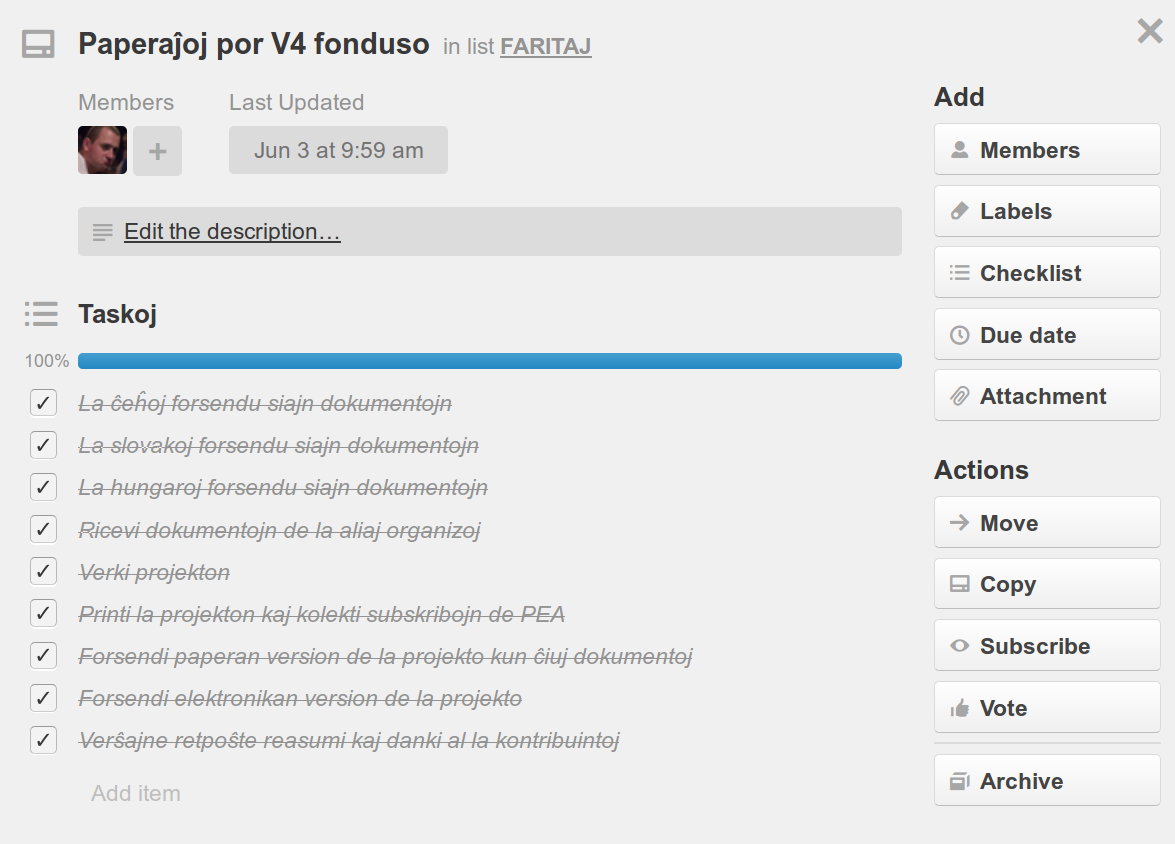
\includegraphics[scale=0.222]{ekranoj/markolistoj}
		\end{center}
	
  \end{frame}
%%%<<<<<<<<<<<<<<<<<<<<<<<<<<<<<<<<<<<<<<<<<<<<<<<<<<<<<<<<<<<<<<<<<<<<<<<<<<<<<<<<<<<<<<<<<<<<<<


%%%>>>>>>>>>>>>>>>>>>>>>>>>>>>>>>>>>>>>>>>>>>>>>>>>>>>>>>>>>>>>>>>>>>>>>>>>>>>>>>>>>>>>>>>>>>>>>>
  \begin{frame}
    \frametitle{Markolistoj + Mencioj}
    \frametitle{Kion ekzemple signifas: klare difinita tasko kun klare difinitaj respondecoj}
    
	\begin{center}
		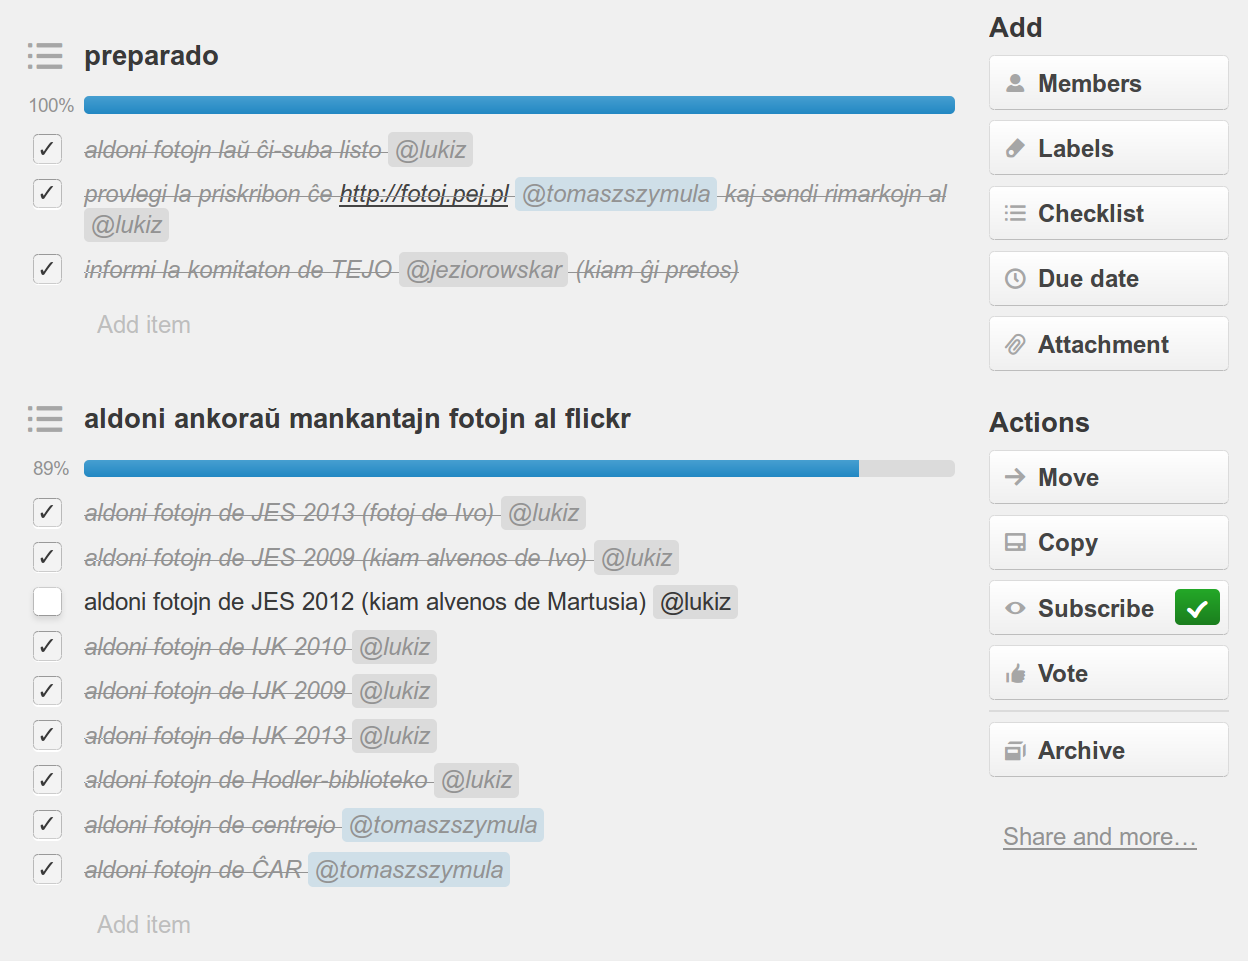
\includegraphics[scale=0.175]{ekranoj/markolistoj-kun-mencioj}
	\end{center}
	
  \end{frame}
%%%<<<<<<<<<<<<<<<<<<<<<<<<<<<<<<<<<<<<<<<<<<<<<<<<<<<<<<<<<<<<<<<<<<<<<<<<<<<<<<<<<<<<<<<<<<<<<<

%%%>>>>>>>>>>>>>>>>>>>>>>>>>>>>>>>>>>>>>>>>>>>>>>>>>>>>>>>>>>>>>>>>>>>>>>>>>>>>>>>>>>>>>>>>>>>>>>
  \begin{frame}
    \frametitle{Limdatoj}
    \frametitle{Kion ekzemple signifas: klare difinite kiam}

    \begin{columns}
    \column{0.6\textwidth}
    
    Tre utilas. Oni ankaŭ ricevas sciigon unu tago antaŭ ĝi.
        	
	\column{0.4\textwidth}
    
    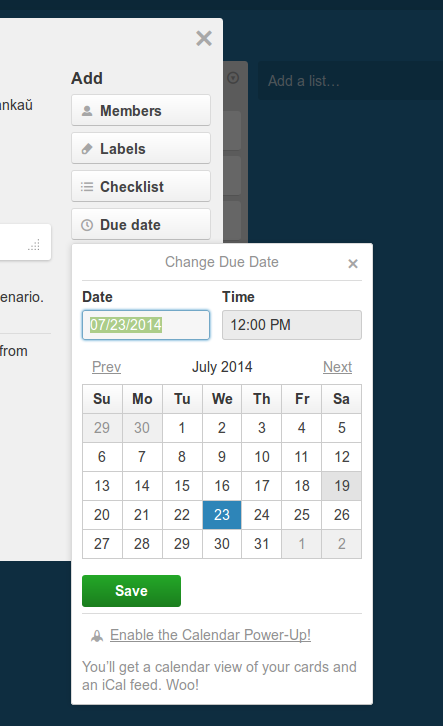
\includegraphics[scale=0.2]{ekranoj/limdato}
	
	\end{columns}
	
	
	
  \end{frame}
%%%<<<<<<<<<<<<<<<<<<<<<<<<<<<<<<<<<<<<<<<<<<<<<<<<<<<<<<<<<<<<<<<<<<<<<<<<<<<<<<<<<<<<<<<<<<<<<<


%%%>>>>>>>>>>>>>>>>>>>>>>>>>>>>>>>>>>>>>>>>>>>>>>>>>>>>>>>>>>>>>>>>>>>>>>>>>>>>>>>>>>>>>>>>>>>>>>
  \begin{frame}
    \frametitle{Etikedoj}
	\framesubtitle{Ne tro uzu}

	\begin{center}
		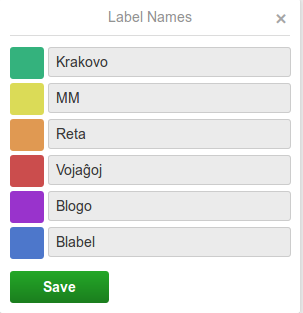
\includegraphics[scale=0.5]{ekranoj/etikedoj}
	\end{center}

  \end{frame}
%%%<<<<<<<<<<<<<<<<<<<<<<<<<<<<<<<<<<<<<<<<<<<<<<<<<<<<<<<<<<<<<<<<<<<<<<<<<<<<<<<<<<<<<<<<<<<<<<



%%%>>>>>>>>>>>>>>>>>>>>>>>>>>>>>>>>>>>>>>>>>>>>>>>>>>>>>>>>>>>>>>>>>>>>>>>>>>>>>>>>>>>>>>>>>>>>>>
  \begin{frame}
    \frametitle{Etikedoj}
	\framesubtitle{Tamen uzu}
	
	
	\begin{center}
		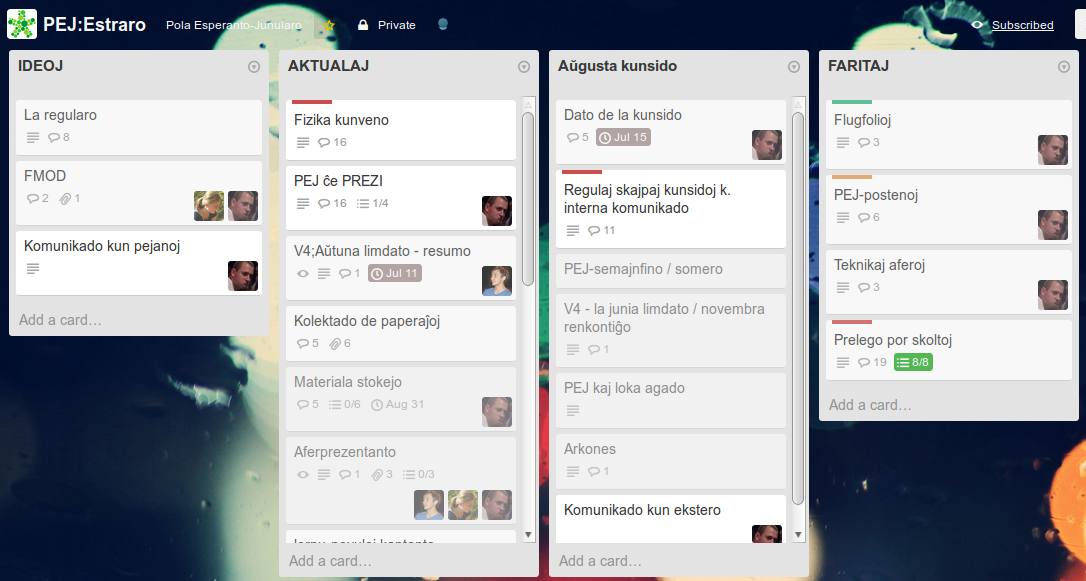
\includegraphics[scale=0.3]{ekranoj/etikedoj-estraro}
	\end{center}

	
  \end{frame}
%%%<<<<<<<<<<<<<<<<<<<<<<<<<<<<<<<<<<<<<<<<<<<<<<<<<<<<<<<<<<<<<<<<<<<<<<<<<<<<<<<<<<<<<<<<<<<<<<


